\subsection{Pengujian Deteksi Pose Pengguna pada Robot di Simulasi}
\label{subsec:deteksiposesimulasi}

Pengujian deteksi pose pengguna pada robot di simulasi dilakukan dengan cara menjalankan lingkungan simulasi yang berisi model pengguna dan menjalankan \emph{pose detector node} yang melakukan proses visi komputer untuk mendeteksi pose dari tangkapan citra model pengguna.
Seperti yang terlihat pada gambar \ref{fig:rosgraphposesimulation},
  \emph{camera plugin} yang ada pada model robot akan mengirimkan tangkapan citra melalui \emph{topic} \lstinline{/camera/image_raw} yang nantinya akan diterima oleh \emph{pose detector node}.

\begin{figure}[ht]
  \centering
  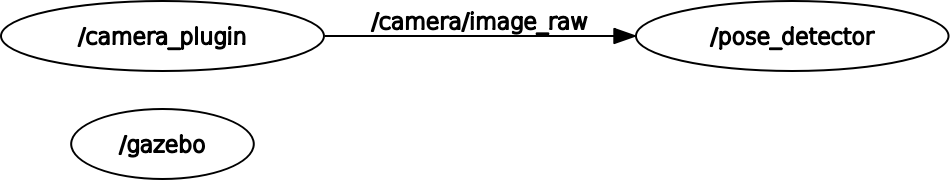
\includegraphics[width=0.95\textwidth,keepaspectratio]{gambar/rosgraph-pose-simulation.png}
  \caption{Relasi antar-\emph{node} dari pengujian deteksi pose pengguna pada robot di simulasi.}
  \label{fig:rosgraphposesimulation}
\end{figure}

Oleh \emph{pose detector node},
  data citra yang diterima tersebut kemudian akan diproses sehingga menghasilkan titik-titik dari setiap bagian pose dari model pengguna.
Titik-titik tersebut kemudian akan digambarkan pada citra yang diproses dan ditampilkan dalam bentuk GUI.
Seperti yang terlihat pada gambar \ref{fig:hasildeteksipose},
  pose yang dideteksi oleh \emph{pose detector node} mampu mendeteksi keseluruhan pose yang membentuk model pengguna.
Pose tersebut juga dapat terdeteksi ketika posisi kaki model pengguna berada dalam kondisi berdiri maupun ditekuk.

\begin{figure}[ht]
  \centering
  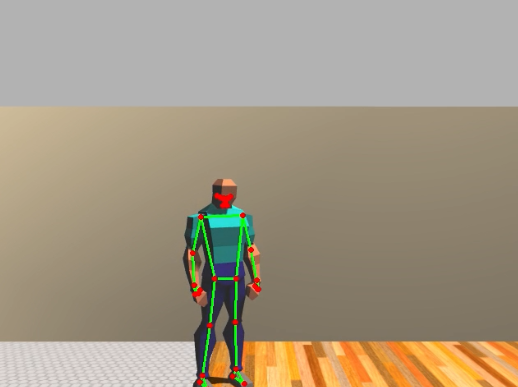
\includegraphics[height=0.35\textwidth,keepaspectratio]{gambar/hasil-deteksi-pose-berdiri.png}
  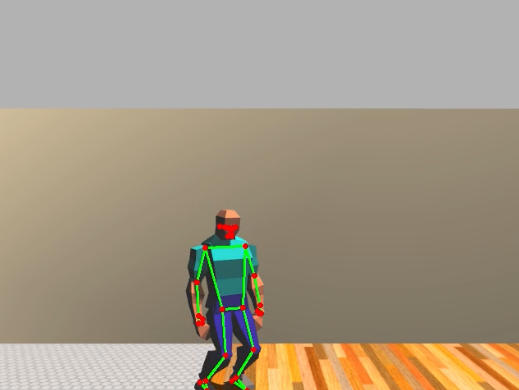
\includegraphics[height=0.35\textwidth,keepaspectratio]{gambar/hasil-deteksi-pose-duduk.png}
  \caption{Hasil deteksi pose pengguna pada robot di simulasi.}
  \label{fig:hasildeteksipose}
\end{figure}
